\documentclass[11pt,journal]{article}
%\usepackage{hyperref}
%\usepackage[breaklinks]{hyperref}
\usepackage{breakurl}
\usepackage{url}
\usepackage{listings}
\usepackage{courier}
\usepackage{amsmath}
\usepackage{graphicx}
\graphicspath{ {/home/agata/Documents/coursework/SensorNetworks/Lab3/} }
%\ifCLASSOPTIONcompsoc
% IEEE Computer Society needs nocompress option
% requires cite.sty v4.0 or later (November 2003)
\usepackage[nocompress]{cite}

%\else
% normal IEEE
\usepackage{cite}
%\fi

\hyphenation{op-tical net-works semi-conduc-tor}
\addtolength{\oddsidemargin}{-.875in}
\addtolength{\evensidemargin}{-.875in} 
\addtolength{\textwidth}{1.75in}

\addtolength{\topmargin}{-.875in}
\addtolength{\textheight}{1.75in}

\begin{document}
	\title{Sensor Networks and Mobile Data Communication, Assignment 3}
	
	\author{UID: 1690550}% <-this % stops a space
		%\protect\\
		%\thanks{}}
	
	% The paper headers



	% IEEEtran.cls defaults to using nonbold math in the Abstract.
	% This preserves the distinction between vectors and scalars. However,
	% if the journal you are submitting to favors bold math in the abstract,
	% then you can use LaTeX's standard command \boldmath at the very start
	% of the abstract to achieve this. Many IEEE journals frown on math
	% in the abstract anyway. In particular, the Computer Society does
	% not want either math or citations to appear in the abstract.
	
	% Note that keywords are not normally used for peerreview papers.
	
	% make the title area
	\maketitle
	
	
	% To allow for easy dual compilation without having to reenter the
	% abstract/keywords data, the \IEEEcompsoctitleabstractindextext text will
	% not be used in maketitle, but will appear (i.e., to be "transported")
	% here as \IEEEdisplaynotcompsoctitleabstractindextext when compsoc mode
	% is not selected <OR> if conference mode is selected - because compsoc
	% conference papers position the abstract like regular (non-compsoc)
	% papers do!
	%\IEEEdisplaynotcompsoctitleabstractindextext
	% \IEEEdisplaynotcompsoctitleabstractindextext has no effect when using
	% compsoc under a non-conference mode.
	
	
	% For peer review papers, you can put extra information on the cover
	% page as needed:
	% \ifCLASSOPTIONpeerreview
	% \begin{center} \bfseries EDICS Category: 3-BBND \end{center}
	% \fi
	%
	% For peerreview papers, this IEEEtran command inserts a page break and
	% creates the second title. It will be ignored for other modes.
	%\IEEEpeerreviewmaketitle
	\section{}
	The three nodes are arranged in the x-y plane, along a single line as follows:
	\begin{figure}[h]
		\centering
		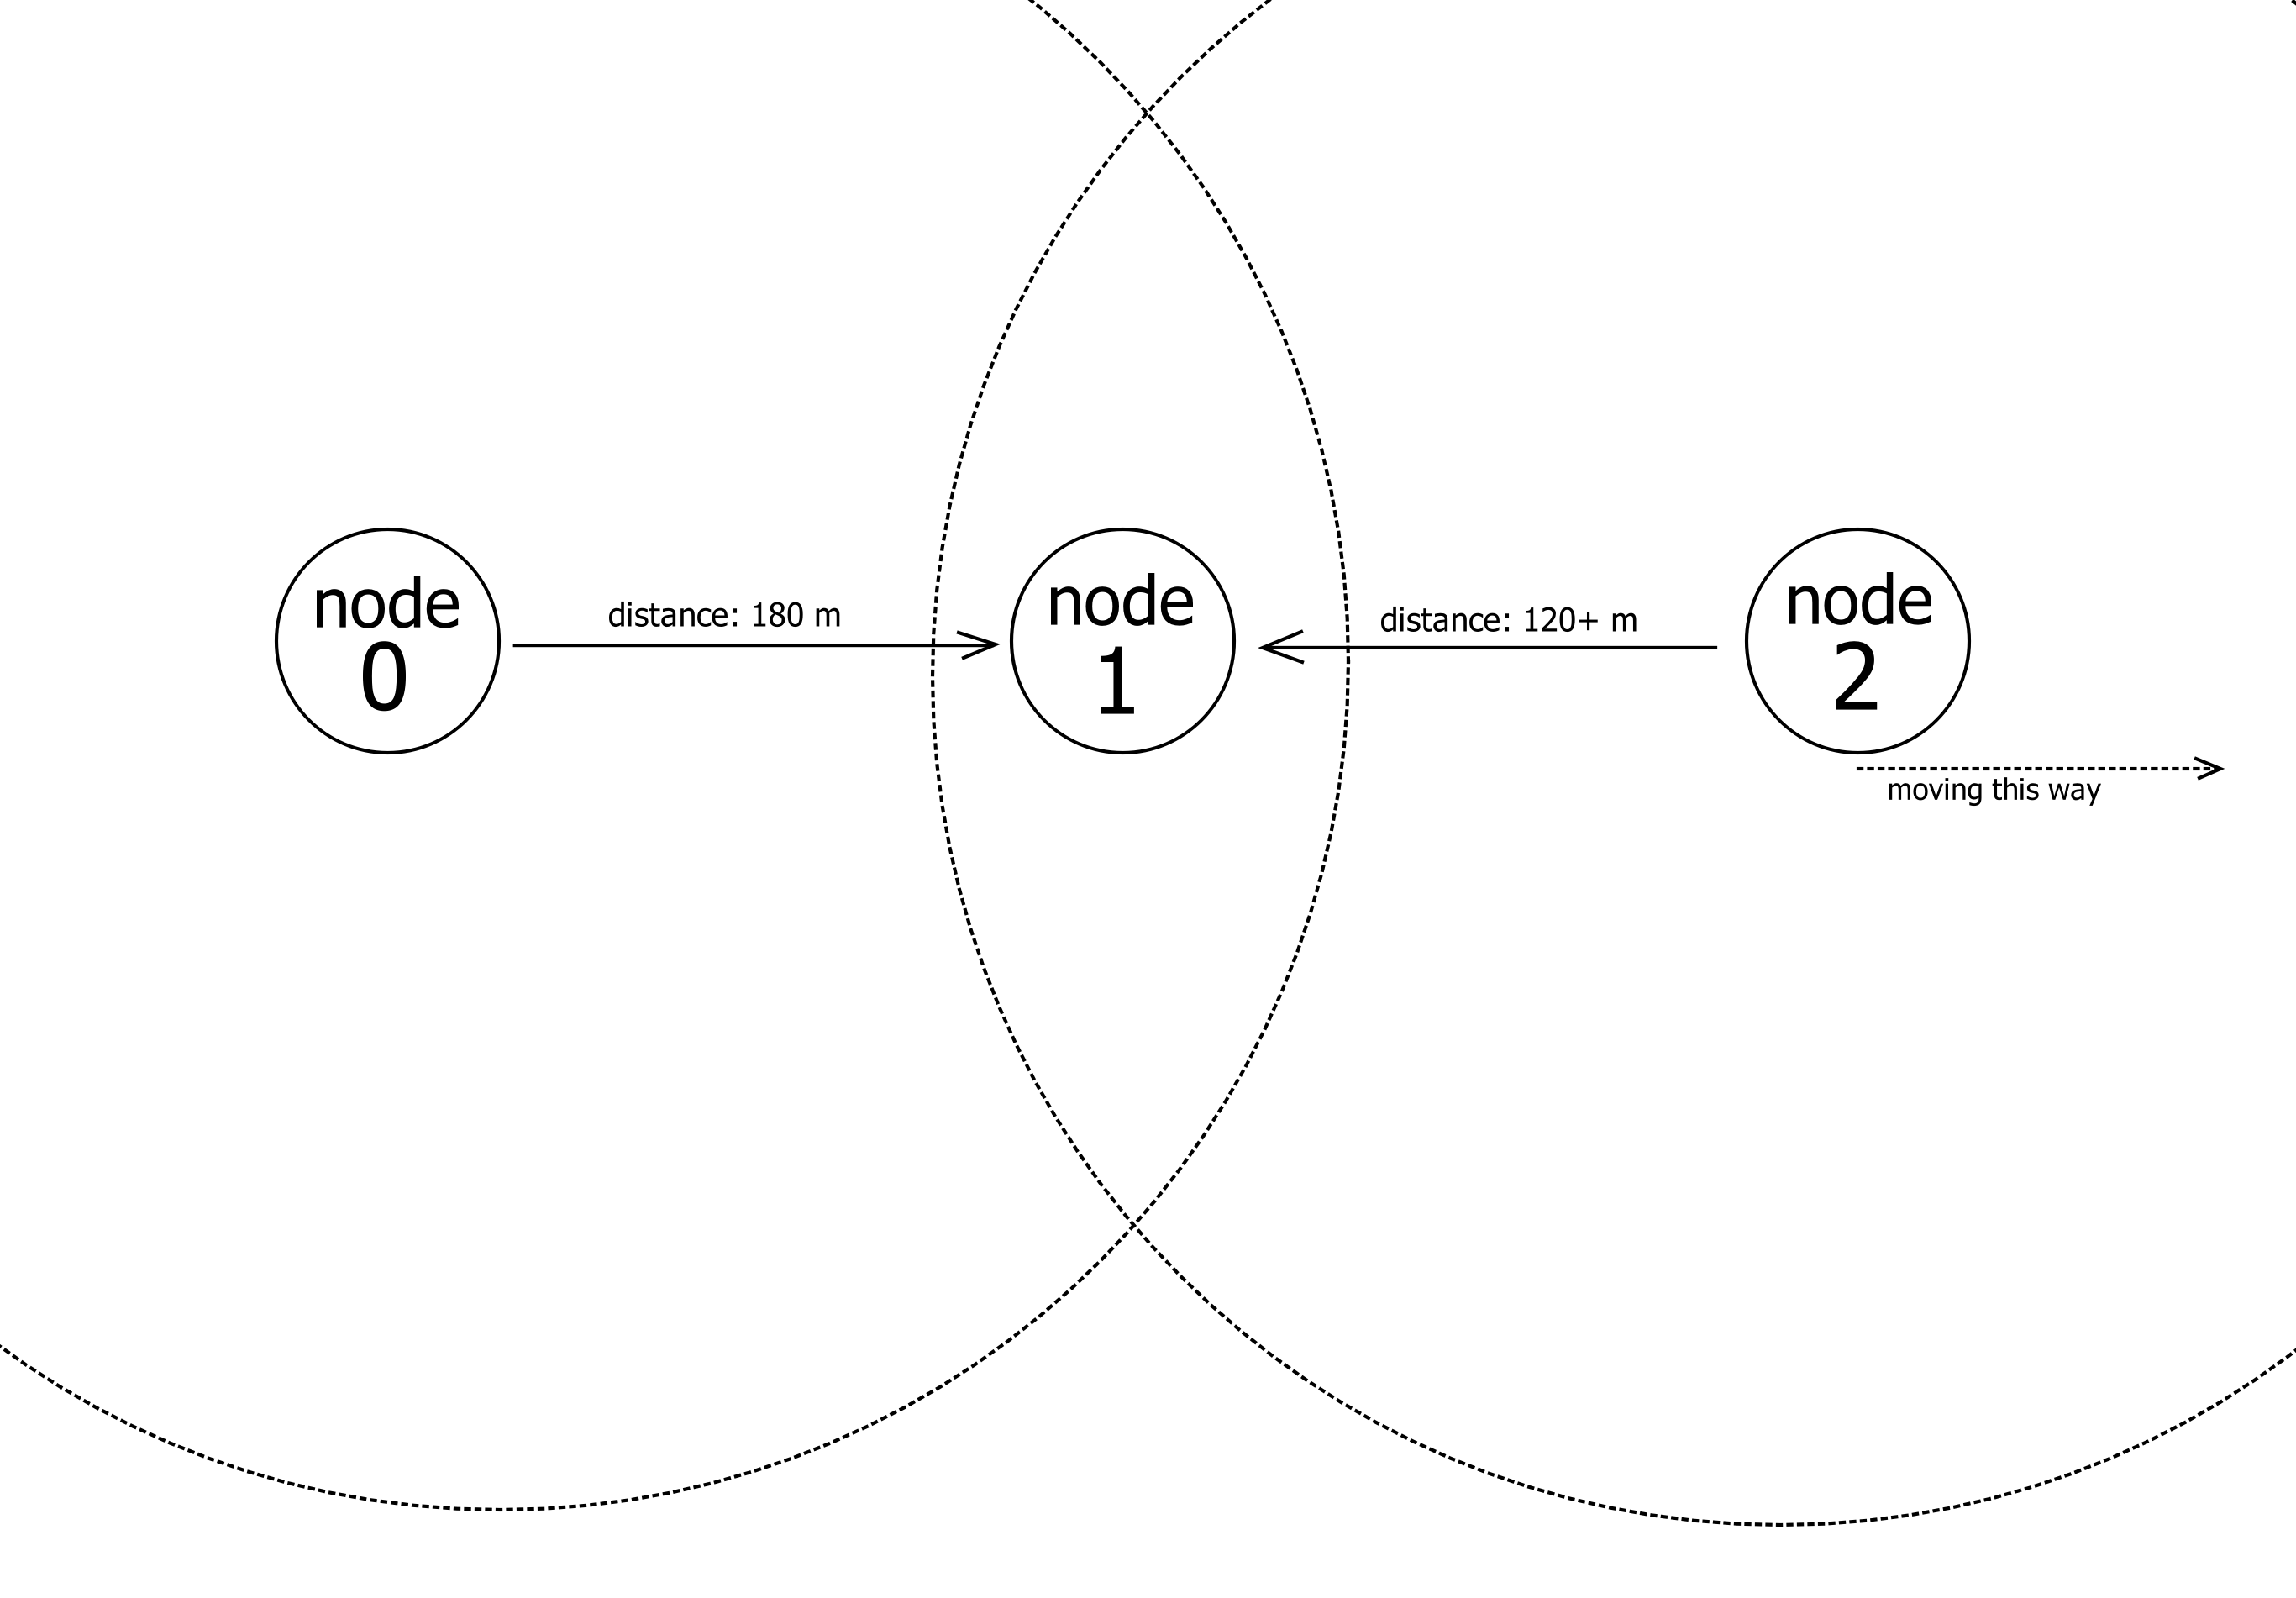
\includegraphics[scale=0.6]{lab3topology2.png}
		\caption{Topology of the network}
	\end{figure}
\pagebreak
	\section{}
	We begin by running the simulation with both Node0 and Node2 generating traffic.
	\begin{figure}[h]
		\centering
		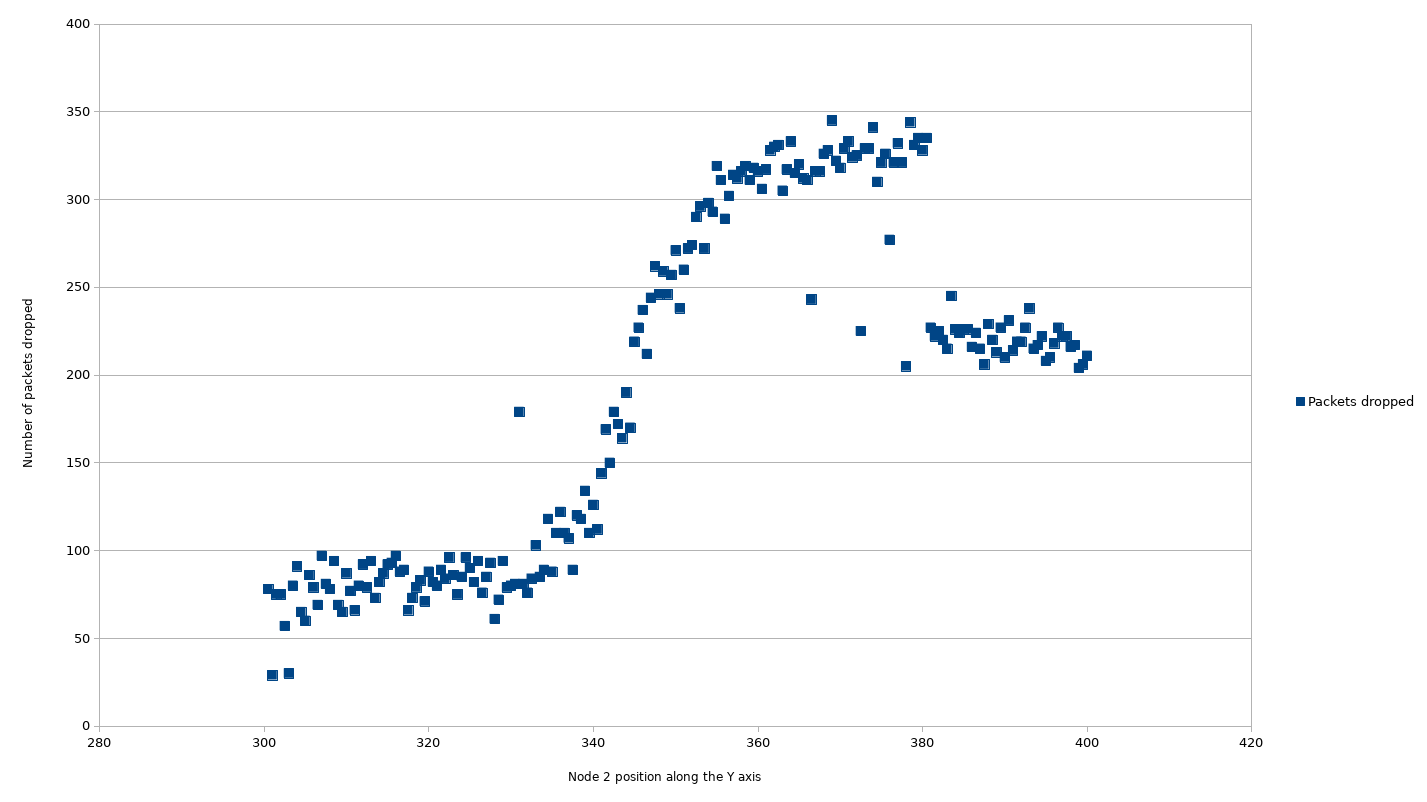
\includegraphics[scale=0.6]{graph1.png}
		\caption{Number of packets dropped plotted against Node2's position on the Y axis}
	\end{figure}

	The number of dropped packets increases as Node2 moves further away from Node1, until it comes outside its range at around 380m mark, after which point we only get packets arriving from Node0. Note that the number of those packets is then constant, following the trend from the second simulation (question 3).
	\pagebreak
	\section{}
	Now we only have Node0 generating traffic.
		
	\begin{figure}[h]
		\centering
		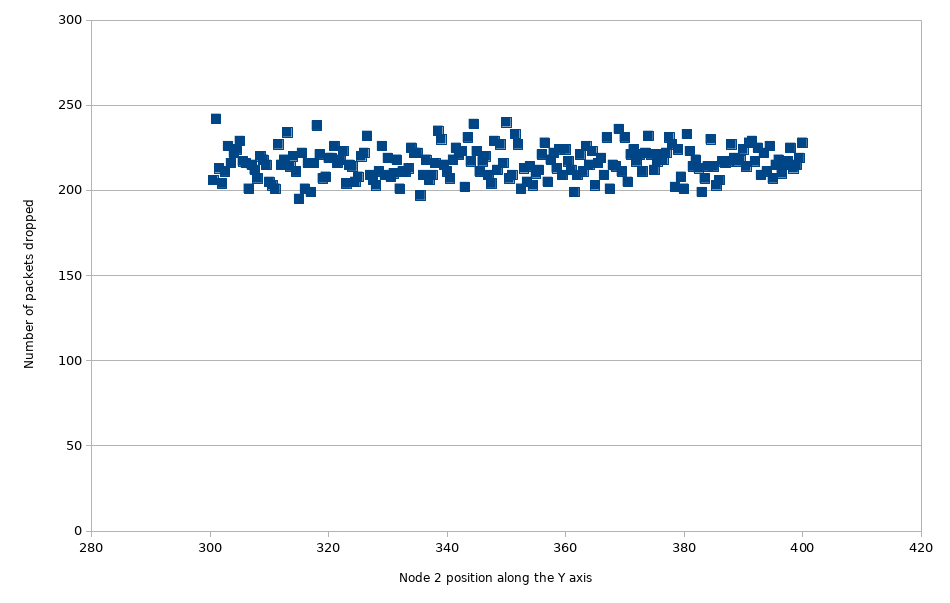
\includegraphics[scale=0.6]{graph2.png}
		\caption{Number of packets dropped plotted against Node2's position on the Y axis, when only Node0 is generating traffic}
	\end{figure}

	As expected, the number of packets dropped stays constant throughout the simulation, because the conditions don't change and there's nothing to affect it.
	
	It is worth noting that the number of packets dropped, averaging at 216, is much higher than at the beginning of the first simulation, due to Node1 not responding with CTS every single time Node0 requested transmission, because Node2 can be transmitting.

	Note that when removing all traffic from Node2 to Node1, we also remove the single packet at the start; otherwise we would get additional 200 packets sent, one for each iteration.
	
	\pagebreak
	\section{}
	We now only have traffic from Node2 to Node1. The number of packets dropped is shown on the graph below.
	\begin{figure}[h]
		\centering
		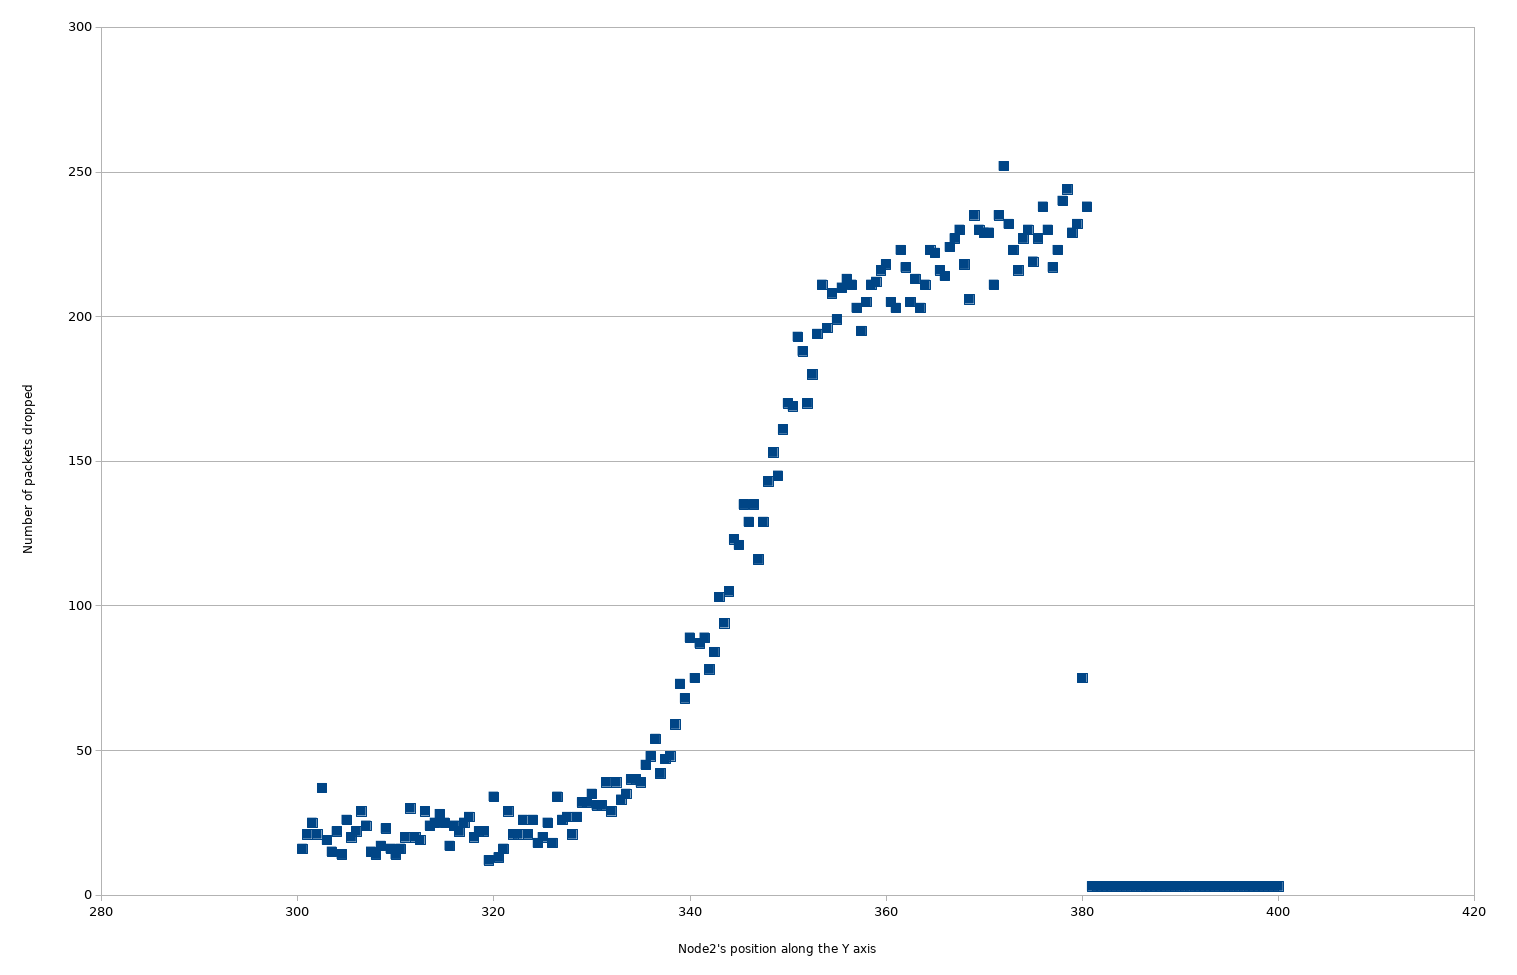
\includegraphics[scale=0.6]{graph3.png}
		\caption{Number of packets dropped plotted against Node2's position on the Y axis, when only Node2 is generating traffic}
	\end{figure}
	
	We can observe that at 360 m mark (180 m from Node1, which is the same as the distance between Node0 and Node1), we see as many packets dropped as in the previous simulation of traffic from Node0 to Node1.
	
	After reaching the distance of 380 m (200 m away from Node1), Node2 moves outside its transmission range, and so no packets can be received by node one. This is reflected by a sudden drop all the way to 0 on the graph. The reason why we see no dropped packages is that even the RTS signals have not been received by Node1, so no packets began transmission.

	As before, we also remove the single packet at the start to initialise the traffic from a node. Otherwise we would get additional 200 packets, one for each iteration.

	\pagebreak
	
	For easier comparison, here are the three graphs plotted together:
		\begin{figure}[h]
			\centering
			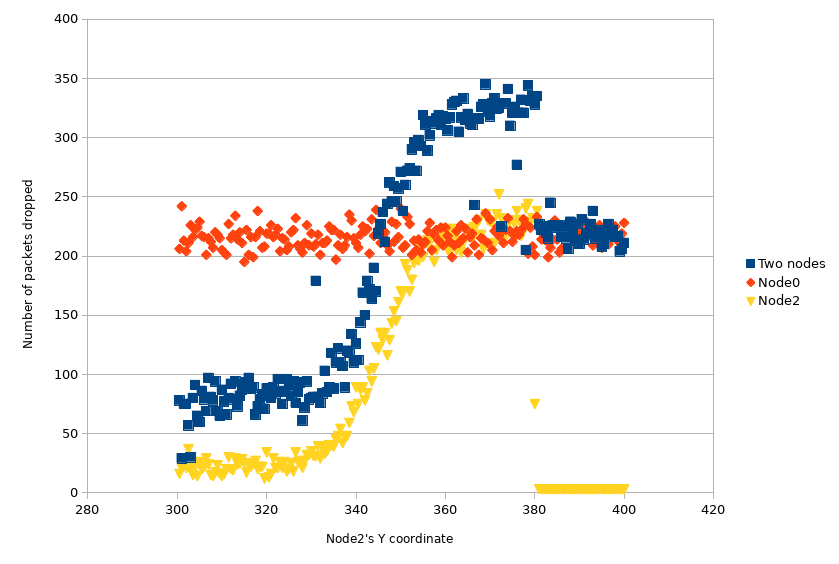
\includegraphics[scale=0.8]{graphall.png}
			\caption{Comparison of the three simulations}
		\end{figure}
	
	\pagebreak
	\section{}
	The original simulation uses packets of size 200 bytes, so we will increase the CTS/RTS limit to 350, thus avoiding any packets sending RTS/CTS. The results plotted against the number of iterations are shown below.
	
	\begin{figure}[h]
		\centering
		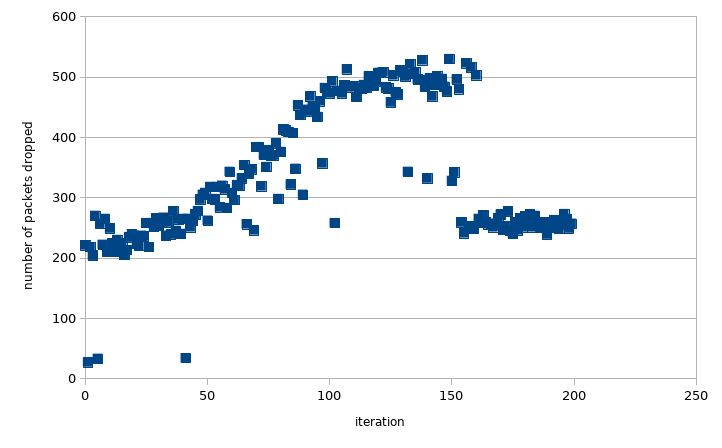
\includegraphics[scale=0.8]{graph5a.png}
		\caption{Number of packets dropped in each iteration}
	\end{figure}

	The shape is very similar to that from the first iterations. To see the differences better, we plot both sets of results together:
	
	\begin{figure}[h]
		\centering
		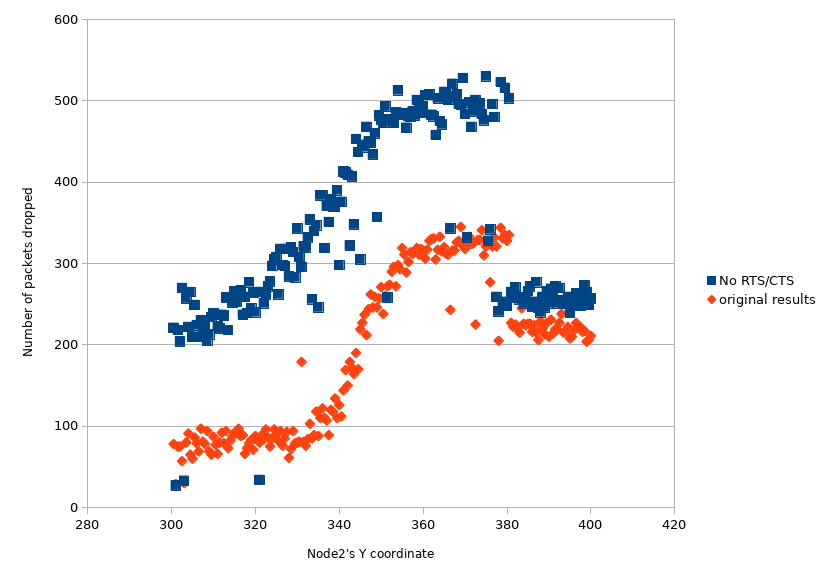
\includegraphics[scale=0.8]{graph5.png}
		\caption{Number of packets dropped, with RTS/CTS and without}
	\end{figure}

	Now we can clearly see that significantly more packets are dropped without the RTS/CTS exchange.
	
	
	
	
	%\IEEEPARstart{}{} 
	

	
	% that's all folks
\end{document}

